\section{Auswertung}

\subsection{Solenoide \label{sec:sol}}

Aus den aufgenommenen Messwerten (s. Anhang) folgen die Abbildungen \ref{fig:kurz} und \ref{fig:lang}.
Bei der langen Spule ist der erwartete Verlauf zu erkennen. Am Beginn der Spule nimmt die Feldstärke zu
und hat dann eine Plateauphase bevor sie am Ende der Spule wieder abfällt.
Der Theoriewert nach Gleichung \eqref{eqn:Solenoid} beträgt $B = \SI{2,432}{\milli \tesla}$.
Bei der kurzen Spule hingegen findet sich zwar ein Maximum, aber es bildet sich kein richtiges Plateu aus,
da nicht mehr $l \gg d$ gilt.
\begin{figure}[H]
  \centering
  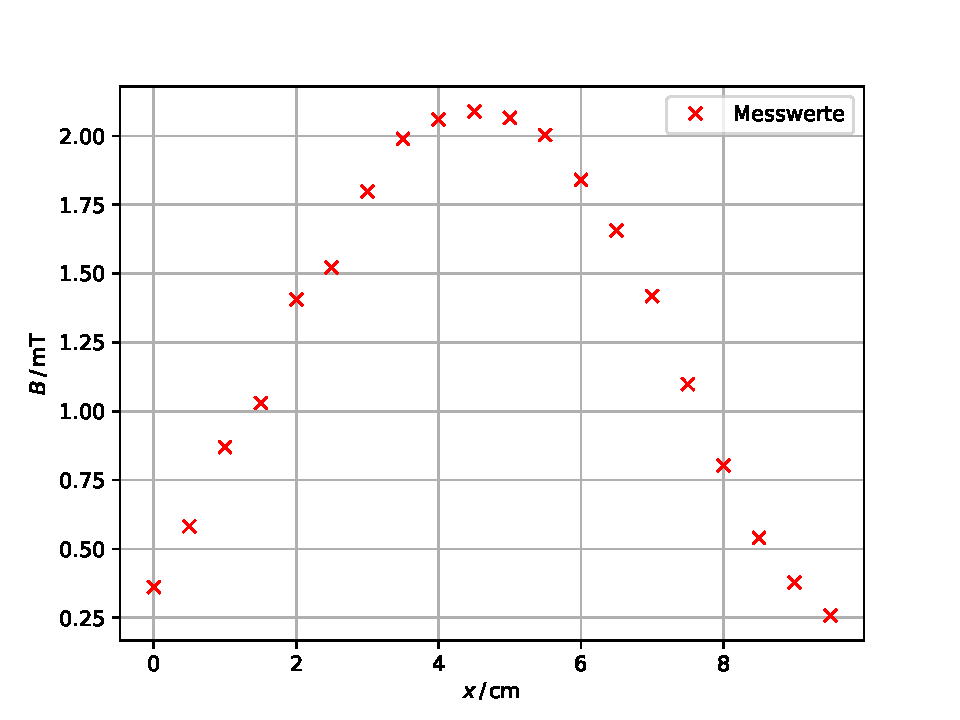
\includegraphics[width=\textwidth]{Plots/kurz.pdf}
  \caption{$B$-$x$-Diagramm zur kurzen Spule}
  \label{fig:kurz}
\end{figure}
\begin{figure}[H]
  \centering
  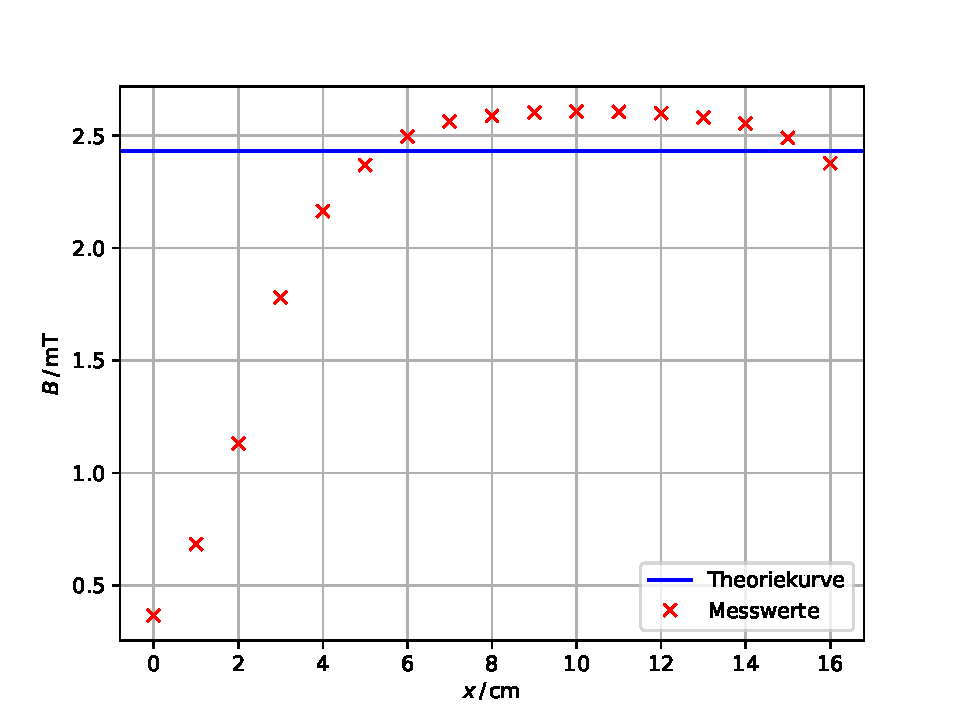
\includegraphics[width=\textwidth]{Plots/lang.pdf}
  \caption{$B$-$x$-Diagramm zur langen Spule}
  \label{fig:lang}
\end{figure}


\subsection{Helmholtz-Spulen \label{sec:helm}}

Die Messwerte sind in den Abbildungen \ref{fig:helm1}, \ref{fig:helm2} und \ref{fig:helm3} aufgetragen.
In Abbildung \ref{fig:helm1}, wo der Abstand ungefähr dem Radius der Helmholtz-Spulen entspricht,
ist das durch Superposition erhaltene homogene Magnetfeld gut zu erkennen.
Der Theoriewert ergibt sich aus Gleichung \eqref{eqn:bfeld} und beträgt $B = \SI{4,006}{\milli \tesla}$.
In den Abbildungen \ref{fig:helm2} und \ref{fig:helm3} wurde der Abstand erhöht und der ideale Fall liegt nicht
mehr vor. Es entsteht kein homogenes Magnetfeld mehr.
Bei einem Abstand von $\SI{9}{\centi \meter}$ beträgt der Theoriewert $B = \SI{3,224}{\milli \tesla}$ und bei
$\SI{11}{\centi \meter}$ ist $B = \SI{2,552}{\milli \tesla}$

\begin{figure}[H]
  \centering
  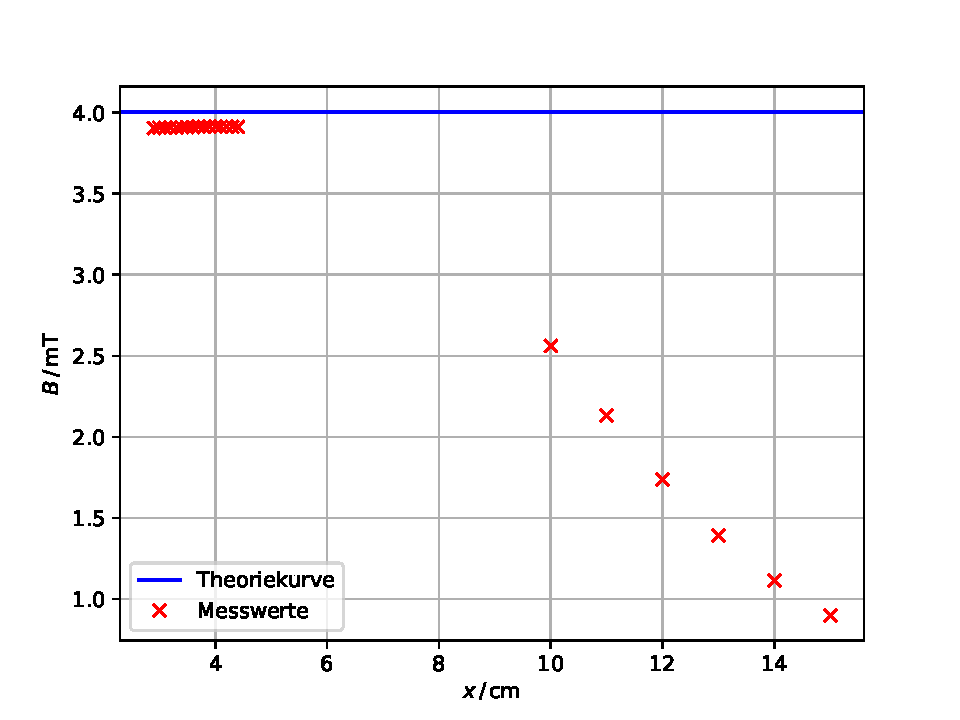
\includegraphics[width=\textwidth]{Plots/helm1.pdf}
  \caption{$B$-$x$-Diagramm für ein Helmholtz-Spulenpaar mit Abstand $d = \SI{7}{\centi \meter}$}
  \label{fig:helm1}
\end{figure}
\begin{figure}[H]
  \centering
  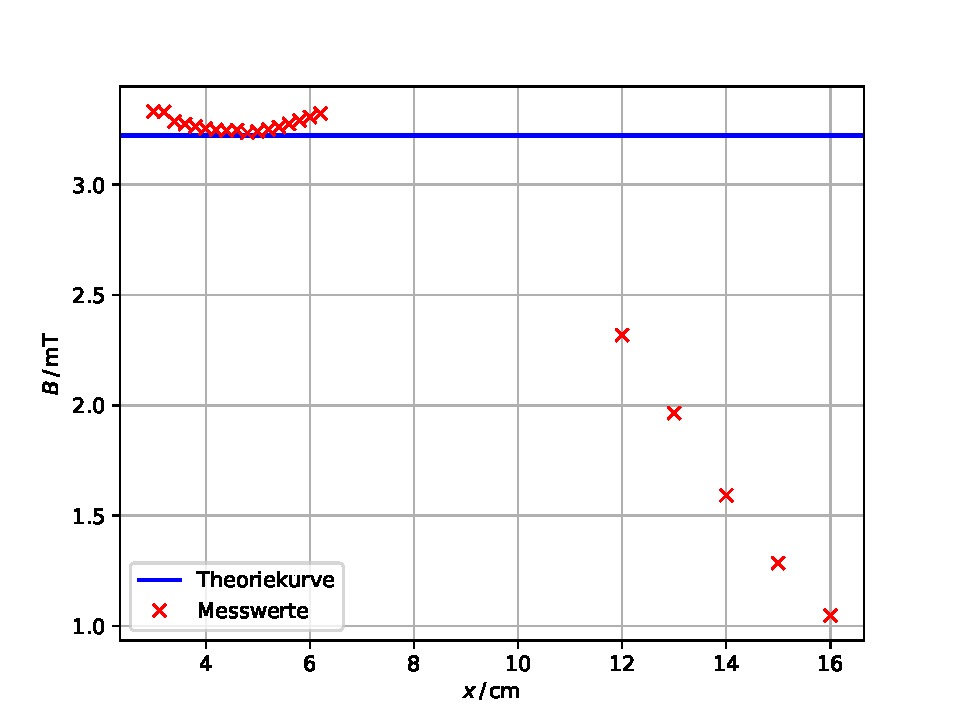
\includegraphics[width=\textwidth]{Plots/helm2.pdf}
  \caption{$B$-$x$-Diagramm für ein Helmholtz-Spulenpaar mit Abstand $d = \SI{9}{\centi \meter}$}
  \label{fig:helm2}
\end{figure}
\begin{figure}[H]
  \centering
  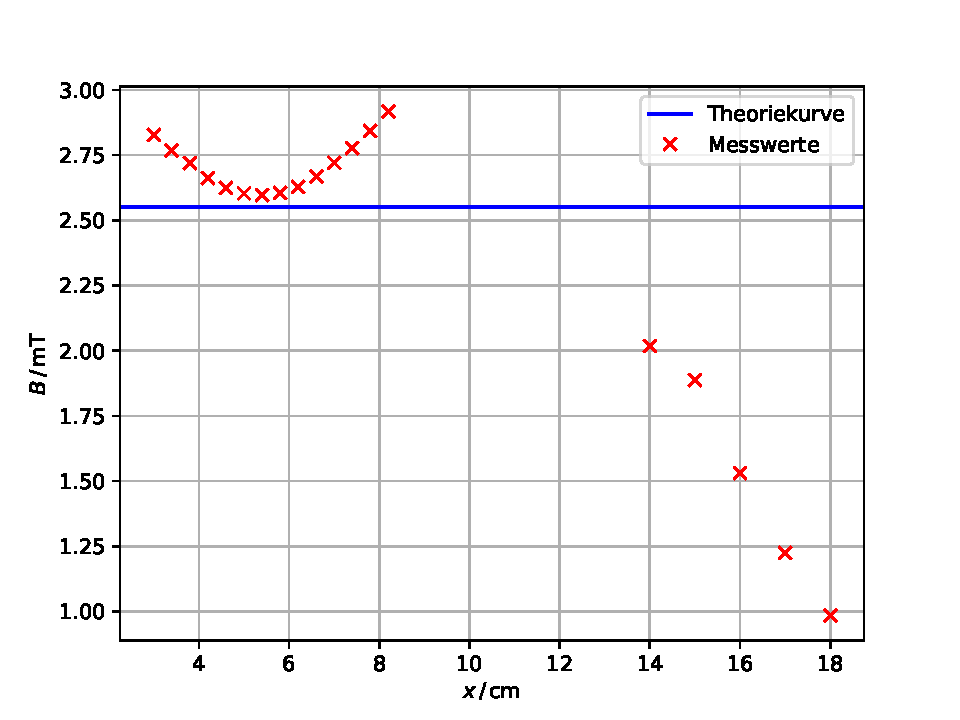
\includegraphics[width=\textwidth]{Plots/helm3.pdf}
  \caption{$B$-$x$-Diagramm für ein Helmholtz-Spulenpaar mit Abstand $d = \SI{11}{\centi \meter}$}
  \label{fig:helm3}
\end{figure}


\subsection{Toroid \label{sec:hys}}

Aus der Hysteresekurve in Abbildung \ref{fig:torus} lassen sich die Werte
\begin{align*}
  B_S &= \SI{706,65}{\milli \tesla} \\
  B_r &= \SI{91,7}{\milli \tesla} \\
  I_c &= \SI{-0,55}{\A}
\end{align*}

ablesen.
Dies sind die Sättigungsmagnetisierung $B_S$, die Remanenz $B_r$ und das Äquvivalent zur Koerzitivkraft $H_c$.
Anhand der schmalen Hystereschleife lässt sich erkennen, dass es sich in diesem Fall um ein magnetisch weiches
Material handelt.
\begin{figure}[H]
  \centering
  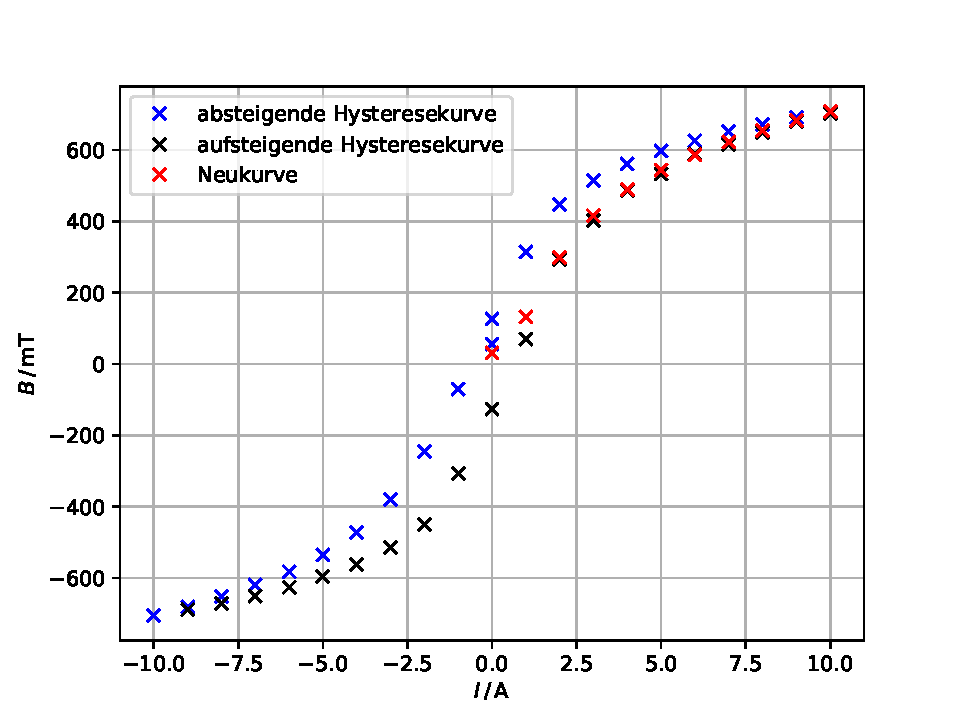
\includegraphics[width=\textwidth]{Plots/torus.pdf}
  \caption{$B$-$I$-Diagramm mit Hysteresekurve für eine Toroidspule}
  \label{fig:torus}
\end{figure}
